\section{Register Interface and Bus State Logic}

The I2C core (also known as the Two-Wire Interface, TWI) is controlled via a set of memory-mapped registers. These
registers configure and monitor both the Master and Slave functionalities. In addition to the register details, the core
includes a state machine that continuously monitors bus activity. The following sections detail the registers, their bit-level
descriptions, and the bus state logic.

\subsection{Overview of Bus State Logic}

The I2C bus state logic is responsible for monitoring the activity on the SDA and SCL lines to determine the current state
of the bus. The bus state can be one of the following:

\begin{itemize}
  \item \textbf{UNKNOWN:} The bus state is undefined, such as immediately after reset.
  \item \textbf{IDLE:} The bus is inactive. No Start condition has been detected.
  \item \textbf{OWNER:} The I2C core is the current master and controls the bus.
  \item \textbf{BUSY:} The bus is active, either due to a Start condition generated externally or because the master has lost
      arbitration.
\end{itemize}

\paragraph{Block Diagram:}  
Figure~\ref{fig:i2c_block_diagram} illustrates a simplified block diagram of the I2C core including the bus state logic.
This logic monitors SDA and SCL, detects Start/Stop conditions, and signals events such as collisions or time-outs.

\begin{figure}[H]
    \centering
    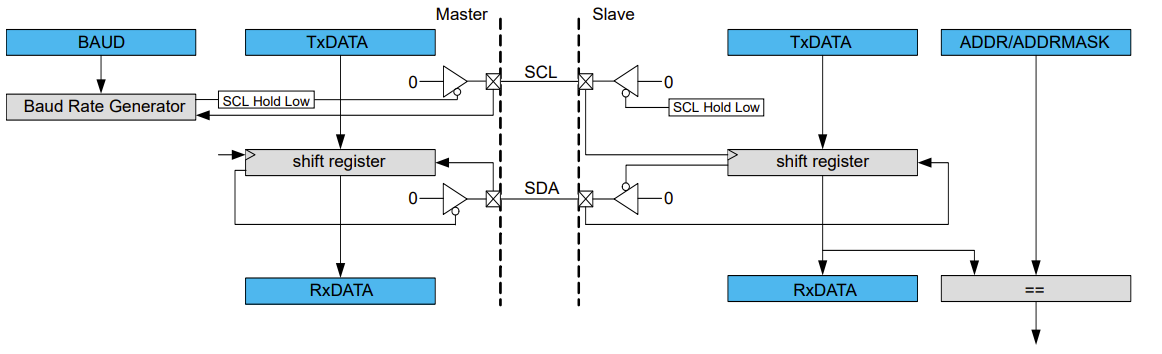
\includegraphics[width=0.75\textwidth]{images/i2c_block_diagram.png}  % Replace with actual image
    \caption{Simplified I2C Block Diagram Including Bus State Logic}
    \label{fig:i2c_block_diagram}
\end{figure}

The bus state is reported in the \texttt{BUSSTATE} field of the Master Status register (\texttt{MSTATUS}). Software
can poll this field or use interrupts to detect transitions (e.g. from IDLE to BUSY) and to reinitialize communications
appropriately after collisions or unexpected bus errors.

\bigskip

\subsection{Register Summary}

The following table summarizes the registers used by the I2C core and their corresponding addresses (assuming an 8-bit data
width configuration):

\renewcommand*{\arraystretch}{1.4}
\begingroup
\small
\rowcolors{2}{gray!30}{gray!10}
\begin{longtable}[H]{
    | p{0.25\textwidth}
    | p{0.15\textwidth}
    | p{0.55\textwidth} |
  }
  \hline
  \rowcolor{black}
  \textcolor{white}{\textbf{Register Name}} &
  \textcolor{white}{\textbf{Address}} &
  \textcolor{white}{\textbf{Description}} \\ \hline \hline
  \endfirsthead
  
  \rowcolor{black}
  \textcolor{white}{\textbf{Register Name}} &
  \textcolor{white}{\textbf{Address}} &
  \textcolor{white}{\textbf{Description}} \\ \hline \hline
  \endhead
  
  \hline
  \endfoot
  
  MCTRLA  & 0x00 & Master Control A: Configures master operation, enables interrupts, and sets bus timeout. \\ \hline
  MSTATUS & 0x01 & Master Status: Reports the master transfer status and bus state. \\ \hline
  MBAUD   & 0x02 & Master Baud: Sets the clock prescaler for SCL generation. \\ \hline
  MADDR   & 0x03 & Master Address: Contains the target slave address and R/W bit for initiating transactions. \\ \hline
  MDATA   & 0x04 & Master Data: Used for transmitting or receiving data bytes in master mode. \\ \hline
  SCTRLA  & 0x05 & Slave Control A: Configures slave operation, including address recognition and smart mode. \\ \hline
  SSTATUS & 0x06 & Slave Status: Reports the status of slave operations, such as data reception, collisions, or errors. \\ \hline
  SADDR   & 0x07 & Slave Address: Configures the slave address and general call recognition. \\ \hline
  SDATA   & 0x08 & Slave Data: Used for transmitting or receiving data bytes in slave mode. \\ \hline
  \caption{I2C Core Register Summary}
  \label{table:i2c_register_summary}
\end{longtable}
\endgroup

\subsection{Detailed Register Descriptions}

In the following sections, each register is described in detail.

\subsubsection{Master Control A (\texttt{MCTRLA})}
\label{sec:mctrla}

\textbf{Address:} \texttt{0x00} \\
\textbf{Default value:} 0x00

\paragraph{Description:}  
The \texttt{MCTRLA} register configures the I2C master operation. It enables the master block, selects the bus
timeout period, and configures the interrupt sources for both read and write operations. When enabled, the master
controls the clock (SCL) and initiates transactions via Start conditions.

\paragraph{Bit Fields:}
\begin{itemize}[leftmargin=*,itemsep=2mm]
  \item \textbf{Bit 7: RIEN (Read Interrupt Enable)}  
        \begin{itemize}
          \item \texttt{0}: Read interrupt disabled.
          \item \texttt{1}: Read interrupt enabled; sets the \texttt{RIF} flag in \texttt{MSTATUS} upon read completion.
        \end{itemize}
  \item \textbf{Bit 6: WIEN (Write Interrupt Enable)}  
        \begin{itemize}
          \item \texttt{0}: Write interrupt disabled.
          \item \texttt{1}: Write interrupt enabled; sets the \texttt{WIF} flag in \texttt{MSTATUS} after transmission.
        \end{itemize}
  \item \textbf{Bit 5: QCEN (Quick Command Enable)}  
        \begin{itemize}
          \item \texttt{0}: Quick Command mode is disabled.
          \item \texttt{1}: Quick Command mode enabled for SMBus operations (sends only an address and R/W bit, no data).
        \end{itemize}
  \item \textbf{Bits 4--3: TIMEOUT[1:0]}  
        \begin{itemize}
          \item Configures the inactive bus timeout period. A nonzero setting forces the bus to transition to IDLE
                if inactivity persists.
        \end{itemize}
  \item \textbf{Bit 2: SMEN (Smart Mode Enable)}  
        \begin{itemize}
          \item \texttt{0}: Smart mode disabled.
          \item \texttt{1}: Smart mode enabled; automatically issues an ACK after reading from \texttt{MDATA}.
        \end{itemize}
  \item \textbf{Bit 1: Reserved}  
        \begin{itemize}
          \item Must be set to \texttt{0}.
        \end{itemize}
  \item \textbf{Bit 0: ENABLE}  
        \begin{itemize}
          \item \texttt{0}: I2C Master disabled.
          \item \texttt{1}: I2C Master enabled.
        \end{itemize}
\end{itemize}

\paragraph{Usage Example:}  
To enable the I2C master for Fast mode (400 kHz) with smart mode and both read/write interrupts active, software could write:
\begin{verbatim}
MCTRLA = 0b1_1_1_XX_1_0_1;  // Replace XX with proper TIMEOUT bits
\end{verbatim}

\vspace{2mm}

\subsubsection{Master Status (\texttt{MSTATUS})}
\label{sec:mstatus}

\textbf{Address:} \texttt{0x01} \\
\textbf{Default value:} 0x00

\paragraph{Description:}  
The read-only \texttt{MSTATUS} register provides real-time status information for the master operation. It includes flags that
indicate the completion of read or write operations, whether the master is currently holding the clock, if a slave has not
acknowledged, and the current bus state (as determined by the bus state logic).

\paragraph{Bit Fields:}
\begin{itemize}[leftmargin=*,itemsep=2mm]
  \item \textbf{Bit 7: RIF (Read Interrupt Flag)}  
        \begin{itemize}
          \item Set when a byte has been successfully received.
          \item Cleared by reading \texttt{MSTATUS} and then \texttt{MDATA}, or by writing a '1' to the bit.
        \end{itemize}
  \item \textbf{Bit 6: WIF (Write Interrupt Flag)}  
        \begin{itemize}
          \item Set when a write transaction has completed.
          \item Cleared via reading the register or by writing a '1' to the bit.
        \end{itemize}
  \item \textbf{Bit 5: CLKHOLD}  
        \begin{itemize}
          \item Indicates that SCL is held low (due to clock stretching, for example).
        \end{itemize}
  \item \textbf{Bit 4: RXACK (Received Acknowledge)}  
        \begin{itemize}
          \item \texttt{0}: Slave ACK received.
          \item \texttt{1}: Slave NACK received.
        \end{itemize}
  \item \textbf{Bit 3: ARBLOST (Arbitration Lost)}  
        \begin{itemize}
          \item Set if the master loses bus arbitration.
          \item Cleared by a software reset (e.g., writing to \texttt{MADDR}).
        \end{itemize}
  \item \textbf{Bit 2: BUSERR (Bus Error)}  
        \begin{itemize}
          \item Signals an illegal bus condition (e.g., an unexpected Stop).
          \item Cleared by specific software actions.
        \end{itemize}
  \item \textbf{Bits 1--0: BUSSTATE}  
        \begin{itemize}
          \item Reports the current bus state as determined by the bus state logic:
                \begin{itemize}
                  \item \texttt{00}: UNKNOWN
                  \item \texttt{01}: IDLE
                  \item \texttt{10}: OWNER
                  \item \texttt{11}: BUSY
                \end{itemize}
        \end{itemize}
\end{itemize}

\vspace{2mm}

\subsubsection{Master Baud (\texttt{MBAUD})}
\label{sec:mbaud}

\textbf{Address:} \texttt{0x02} \\
\textbf{Default value:} 0x00

\paragraph{Description:}  
The \texttt{MBAUD} register determines the SCL clock frequency used by the master. The register value is used as a
divider for the main clock such that the SCL frequency is calculated by:
\[
f_{SCL} = \frac{f_{CLK}}{(2 \cdot \text{BAUD} + C)}
\]
where \(C\) is a design constant. Adjust the \texttt{MBAUD} value to achieve the desired I2C bus speed for Standard,
Fast, or Fast+ modes.

\paragraph{Bit Field:}
\begin{itemize}[leftmargin=*,itemsep=2mm]
  \item \textbf{Bits 7:0: BAUD[7:0]}  
        \begin{itemize}
          \item Directly sets the division factor for SCL generation.
        \end{itemize}
\end{itemize}

\vspace{2mm}

\subsubsection{Master Address (\texttt{MADDR})}
\label{sec:maddr}

\textbf{Address:} \texttt{0x03} \\
\textbf{Default value:} 0x00

\paragraph{Description:}  
The \texttt{MADDR} register holds the target slave address and the read/write direction bit. Writing to this register
initiates a Start condition and begins the address phase of a transaction.

\paragraph{Bit Fields:}
\begin{itemize}[leftmargin=*,itemsep=2mm]
  \item \textbf{Bits 7:1: ADDR[7:1]}  
        \begin{itemize}
          \item Contains the 7-bit slave address.
        \end{itemize}
  \item \textbf{Bit 0: R/W}  
        \begin{itemize}
          \item \texttt{0}: Write transaction.
          \item \texttt{1}: Read transaction.
        \end{itemize}
\end{itemize}

\vspace{2mm}

\subsubsection{Master Data (\texttt{MDATA})}
\label{sec:mdata}

\textbf{Address:} \texttt{0x04} \\
\textbf{Default value:} 0x00

\paragraph{Description:}  
The \texttt{MDATA} register is used to transmit data bytes out to the slave and to receive data from the slave.
In master mode, a write operation to this register starts the transmission of the data byte, while a read operation
retrieves the last byte received. Note that \texttt{MDATA} is logically mapped to internal shift registers and buffers.

\paragraph{Bit Field:}
\begin{itemize}[leftmargin=*,itemsep=2mm]
  \item \textbf{Bits 7:0: DATA[7:0]}  
        \begin{itemize}
          \item The data byte to be transmitted, or the data byte received from the slave.
        \end{itemize}
\end{itemize}

\vspace{2mm}

\subsubsection{Slave Control A (\texttt{SCTRLA})}
\label{sec:sctrla}

\textbf{Address:} \texttt{0x05} \\
\textbf{Default value:} 0x00

\paragraph{Description:}  
The \texttt{SCTRLA} register configures the slave functions of the I2C core. It is used to enable the slave block,
configure address recognition features (such as promiscuous mode), and enable interrupts for address or data events.
When enabled, the slave monitors the bus for its address and responds appropriately.

\paragraph{Bit Fields:}
\begin{itemize}[leftmargin=*,itemsep=2mm]
  \item \textbf{Bit 7: DIEN (Data Interrupt Enable)}  
        \begin{itemize}
          \item \texttt{0}: Data interrupt disabled.
          \item \texttt{1}: Data interrupt enabled; the \texttt{DIF} flag in \texttt{SSTATUS} will be set when a transfer completes.
        \end{itemize}
  \item \textbf{Bit 6: APIEN (Address/Stop Interrupt Enable)}  
        \begin{itemize}
          \item \texttt{0}: Address/Stop interrupt disabled.
          \item \texttt{1}: Address/Stop interrupt enabled; the \texttt{APIF} flag is set on address match or Stop condition.
        \end{itemize}
  \item \textbf{Bit 5: PIEN (Stop Interrupt Enable)}  
        \begin{itemize}
          \item \texttt{0}: Stop condition interrupt disabled.
          \item \texttt{1}: Stop condition interrupt enabled.
        \end{itemize}
  \item \textbf{Bit 4: PMEN (Promiscuous Mode/Address Mask Enable)}  
        \begin{itemize}
          \item \texttt{0}: Only the slave address configured in \texttt{SADDR} is recognized.
          \item \texttt{1}: The slave responds to any address or uses a mask (if supported).
        \end{itemize}
  \item \textbf{Bit 3: SMEN (Smart Mode Enable)}  
        \begin{itemize}
          \item \texttt{0}: Smart mode disabled.
          \item \texttt{1}: Smart mode enabled; the slave automatically issues an ACK when \texttt{SDATA} is read.
        \end{itemize}
  \item \textbf{Bits 2--1: Reserved}  
        \begin{itemize}
          \item Must be written as \texttt{0}.
        \end{itemize}
  \item \textbf{Bit 0: ENABLE}  
        \begin{itemize}
          \item \texttt{0}: I2C Slave disabled.
          \item \texttt{1}: I2C Slave enabled.
        \end{itemize}
\end{itemize}

\vspace{2mm}

\subsubsection{Slave Status (\texttt{SSTATUS})}
\label{sec:sstatus}

\textbf{Address:} \texttt{0x06} \\
\textbf{Default value:} 0x00

\paragraph{Description:}  
The \texttt{SSTATUS} register provides status information for the slave side of the I2C core. It indicates data transfer
completion, collisions, bus errors, and provides information on the type of transaction the slave is involved in.

\paragraph{Bit Fields:}
\begin{itemize}[leftmargin=*,itemsep=2mm]
  \item \textbf{Bit 7: DIF (Data Interrupt Flag)}  
        \begin{itemize}
          \item Set when a byte is successfully transferred.
          \item Cleared by reading \texttt{SDATA} or issuing a slave command.
        \end{itemize}
  \item \textbf{Bit 6: APIF (Address/Stop Interrupt Flag)}  
        \begin{itemize}
          \item Set when an address match occurs or a Stop condition is detected.
        \end{itemize}
  \item \textbf{Bit 5: CLKHOLD}  
        \begin{itemize}
          \item Indicates that the slave is holding SCL low (for example, during clock stretching).
        \end{itemize}
  \item \textbf{Bit 4: RXACK (Received Acknowledge)}  
        \begin{itemize}
          \item \texttt{0}: The master has acknowledged the transmitted byte.
          \item \texttt{1}: No acknowledgement received.
        \end{itemize}
  \item \textbf{Bit 3: COLL (Collision)}  
        \begin{itemize}
          \item Set if a collision is detected during data transmission.
          \item Cleared by reading \texttt{SSTATUS} or writing a ‘1’ to this bit.
        \end{itemize}
  \item \textbf{Bit 2: BUSERR (Bus Error)}  
        \begin{itemize}
          \item Indicates detection of an illegal bus condition.
          \item Cleared by software after handling the error.
        \end{itemize}
  \item \textbf{Bit 1: DIR (Direction)}  
        \begin{itemize}
          \item \texttt{0}: Master write operation (slave received data).
          \item \texttt{1}: Master read operation (slave transmits data).
        \end{itemize}
  \item \textbf{Bit 0: AP (Address/Stop)}  
        \begin{itemize}
          \item Distinguishes whether the \texttt{APIF} event was caused by address recognition (\texttt{1})
                or by a Stop condition (\texttt{0}).
        \end{itemize}
\end{itemize}

\vspace{2mm}

\subsubsection{Slave Address (\texttt{SADDR})}
\label{sec:saddr}

\textbf{Address:} \texttt{0x07} \\
\textbf{Default value:} 0x00

\paragraph{Description:}  
The \texttt{SADDR} register holds the slave address that the I2C core monitors on the bus. The upper 7 bits contain
the address, while the least significant bit configures whether the general call address (0x00) should be recognized.

\paragraph{Bit Fields:}
\begin{itemize}[leftmargin=*,itemsep=2mm]
  \item \textbf{Bits 7:1: ADDR[7:1]}  
        \begin{itemize}
          \item Stores the 7-bit slave address.
        \end{itemize}
  \item \textbf{Bit 0: GCALL}  
        \begin{itemize}
          \item \texttt{0}: General call not recognized.
          \item \texttt{1}: The slave will respond to a general call address.
        \end{itemize}
\end{itemize}

\vspace{2mm}

\subsubsection{Slave Data (\texttt{SDATA})}
\label{sec:sdata}

\textbf{Address:} \texttt{0x08} \\
\textbf{Default value:} 0x00

\paragraph{Description:}  
The \texttt{SDATA} register is used for data transfers in slave mode. Writing to \texttt{SDATA} prepares the data that will
be transmitted to the master. Conversely, reading from \texttt{SDATA} retrieves the data byte received from the master.
This register is logically connected to the internal shift registers and any buffering mechanisms used for slave
operation.

\paragraph{Bit Field:}
\begin{itemize}[leftmargin=*,itemsep=2mm]
  \item \textbf{Bits 7:0: DATA[7:0]}  
        \begin{itemize}
          \item Contains the data byte for slave transmit/receive.
        \end{itemize}
\end{itemize}

\vspace{2mm}

\subsection{Addressing and Register Allocation}

Each register is aligned on an 8-bit boundary. For registers that do not fully consume a byte, the remaining bits are
reserved and should remain as their reset value. The registers described above follow a linear address space:
\begin{itemize}
  \item \texttt{MCTRLA}: 0x00
  \item \texttt{MSTATUS}: 0x01
  \item \texttt{MBAUD}: 0x02
  \item \texttt{MADDR}: 0x03
  \item \texttt{MDATA}: 0x04
  \item \texttt{SCTRLA}: 0x05
  \item \texttt{SSTATUS}: 0x06
  \item \texttt{SADDR}: 0x07
  \item \texttt{SDATA}: 0x08
\end{itemize}

Software should follow the recommended read/modify/write procedures when updating any register, especially for the
status registers that are sensitive to timing or bus events.

\bigskip

This concludes the detailed register interface and bus state logic description for the I2C (TWI) core. The following sections
cover simulation and synthesis aspects.
